%%%%%%%%%%%%%%%%%%%%%%%%%%%%%%%%%%%%%%%%%%%%%%%%%%%%%%%%%%%%%%%%%%%%%%%%%%%%%%%%
% File: memoria.tex
% Created: 2011-11-11-12:55 by Leo Ferres
% Modified:
% 2011-11-11-12:55 by Leo Ferres
%
% This is a LaTeX file intended to serve as the boilerplate code for
% "memorias", masters and PhD thesis in the Department of Computer
% Science at the Universidad de Concepción. The idea is to also
% include information relevant for students, such as tips on the
% document, and generally knowledge about how to write these kinds of
% documents, so check http://www.inf.udec.cl/~leo/fdoc.tex.
%%%%%%%%%%%%%%%%%%%%%%%%%%%%%%%%%%%%%%%%%%%%%%%%%%%%%%%%%%%%%%%%%%%%%%%%%%%%%%%%
\documentclass[12pt]{diicc}

%%%%%%%%%%%%%%%%%%%%%%%%%%%%%%%%%%%%%%%%%%%%%%%%%%%%%%%%%%%%%%%%%%%%%%%%%%%%%%%%
% Step 1: Add your packages here
%
% http://math.kangwon.ac.kr/~yhpark/tex/packages.html
%%%%%%%%%%%%%%%%%%%%%%%%%%%%%%%%%%%%%%%%%%%%%%%%%%%%%%%%%%%%%%%%%%%%%%%%%%%%%%%%
\usepackage{setspace}
\usepackage{graphicx}
\setcounter{secnumdepth}{3}
\usepackage[linesnumbered,ruled,vlined]{algorithm2e}
\usepackage{url}


%%%%%%%%%%%%%%%%%%%%%%%%%%%%%%%%%%%%%%%%%%%%%%%%%%%%%%%%%%%%%%%%%%%%%%%%%%%%%%%%
% Step 2: Un-comment these commands if this is a draft
%
%%%%%%%%%%%%%%%%%%%%%%%%%%%%%%%%%%%%%%%%%%%%%%%%%%%%%%%%%%%%%%%%%%%%%%%%%%%%%%%%
%\draft
%\singlespace

%%%%%%%%%%%%%%%%%%%%%%%%%%%%%%%%%%%%%%%%%%%%%%%%%%%%%%%%%%%%%%%%%%%%%%%%%%%%%%%%
% Step 3: Add your definitions here
%
% http://en.wikibooks.org/wiki/LaTeX/Customizing_LaTeX
%%%%%%%%%%%%%%%%%%%%%%%%%%%%%%%%%%%%%%%%%%%%%%%%%%%%%%%%%%%%%%%%%%%%%%%%%%%%%%%%
\newcommand{\ignore}[1]{}

%%%%%%%%%%%%%%%%%%%%%%%%%%%%%%%%%%%%%%%%%%%%%%%%%%%%%%%%%%%%%%%%%%%%%%%%%%%%%%%%
% Step 4: Choose your degree
% You can write either \eng for Engineering, \msc for Masters and \phd
% for Doctor of Philosophy. Engineering is set as default.
%%%%%%%%%%%%%%%%%%%%%%%%%%%%%%%%%%%%%%%%%%%%%%%%%%%%%%%%%%%%%%%%%%%%%%%%%%%%%%%%
\eng

%%%%%%%%%%%%%%%%%%%%%%%%%%%%%%%%%%%%%%%%%%%%%%%%%%%%%%%%%%%%%%%%%%%%%%%%%%%%%%%%
% Step 5: Choose title and add author
%%%%%%%%%%%%%%%%%%%%%%%%%%%%%%%%%%%%%%%%%%%%%%%%%%%%%%%%%%%%%%%%%%%%%%%%%%%%%%%%
\title{\bf Physical sharing of clauses in parallel SAT solvers}
\author{Juan Luis Olate Hinrichs}

%%%%%%%%%%%%%%%%%%%%%%%%%%%%%%%%%%%%%%%%%%%%%%%%%%%%%%%%%%%%%%%%%%%%%%%%%%%%%%%%
% Step 6: Add your advisor
%%%%%%%%%%%%%%%%%%%%%%%%%%%%%%%%%%%%%%%%%%%%%%%%%%%%%%%%%%%%%%%%%%%%%%%%%%%%%%%%
\advisor{Leonardo Ferres}

%%%%%%%%%%%%%%%%%%%%%%%%%%%%%%%%%%%%%%%%%%%%%%%%%%%%%%%%%%%%%%%%%%%%%%%%%%%%%%%%
% Step 7: Set your submission, copyright and defense dates. 
%
% Notice that these are not typeset. But they do serve a purpose for
% future references.
%%%%%%%%%%%%%%%%%%%%%%%%%%%%%%%%%%%%%%%%%%%%%%%%%%%%%%%%%%%%%%%%%%%%%%%%%%%%%%%%
\submitdate{September, 2011} % date you submitted to the committee
\defensedate{Octubre, 2011}  % date the defense was set
\copyrightyear{2011}         % document for final archiving

\begin{document}
\frontmatter

%%%%%%%%%%%%%%%%%%%%%%%%%%%%%%%%%%%%%%%%%%%%%%%%%%%%%%%%%%%%%%%%%%%%%%%%%%%%%%%%
% Step 8: Acknowledgments and dedication
%
% Uncomment this in the final version
%%%%%%%%%%%%%%%%%%%%%%%%%%%%%%%%%%%%%%%%%%%%%%%%%%%%%%%%%%%%%%%%%%%%%%%%%%%%%%%%
% \begin{acknowledgements}
% .....
% \end{acknowledgements}

% \begin{dedication}
% To my parents, my family, and whomever it may concern...  
% \end{dedication}

%%%%%%%%%%%%%%%%%%%%%%%%%%%%%%%%%%%%%%%%%%%%%%%%%%%%%%%%%%%%%%%%%%%%%%%%%%%%%%%%
% Step 9: Add abstract
%
% http://research.berkeley.edu/ucday/abstract.html
%%%%%%%%%%%%%%%%%%%%%%%%%%%%%%%%%%%%%%%%%%%%%%%%%%%%%%%%%%%%%%%%%%%%%%%%%%%%%%%%
\begin{abstract}
Your abstract goes here...
\end{abstract}

%%%%%%%%%%%%%%%%%%%%%%%%%%%%%%%%%%%%%%%%%%%%%%%%%%%%%%%%%%%%%%%%%%%%%%%%%%%%%%%%
% Step 10: Add an introduction
%
% 
%%%%%%%%%%%%%%%%%%%%%%%%%%%%%%%%%%%%%%%%%%%%%%%%%%%%%%%%%%%%%%%%%%%%%%%%%%%%%%%%
\mainmatter
\chapter{Introduction}\label{chap:intro}

One of the most well-known problems in computer science is the satisfiability (SAT) problem. This is because this was the first problem to be proved to be NP-complete \cite{cook1971}, proof known as the Cook-Levin theorem\footnote[1]{They both proved it independently.}. One year later, in 1972, Karp proved in \cite{karp1972} that many common combinatorial problems could be reduced in polynomial time to instances of the SAT problem, thus drawing even more attention to SAT problems by the scientific community. Because many combinatorial problems can be reduced to SAT, it is not strange to find many practical problems with useful applications (such as circuit design and automatic theorem proving) that could be solved if there was an efficient algorithm to solve the SAT problem. Unfortunately, because of the NP-complete nature of SAT, such algorithm has not been found yet, but also has not been proven to be in-existent. Many researchers suspect such efficient algorithm to solve all SAT instances does not exist, so instead of trying to solve the NP-complete problem, they try to improve the current SAT solving algorithms.Over the years, SAT solvers have shown impressive improvement, the first complete algorithm, the Davis Putnam algorithm \cite{DP1960}, was very limited and could only handle problems with around ten variables. Today, modern SAT solvers can handle instances with millions of variables, making such solvers suitable even for industrial application. In the next chapter we will point out the main features that have improved SAT solvers significantly. 

In the last decade parallel computing has become increasingly popular. As CPU manufacturers have found difficult and expensive to keep increasing the clock speed of processors, they have instead turn to increase the number of cores each chip has. Unfortunately, if the algorithms are not thought to be run in parallel, more cores will bring small improvements. This is the reason why there is a growing concern to parallelize algorithms so that they can take advantage of many-cores architectures of today's computers. In SAT solving it is no different. The annual SAT competition \footnote[1]{www.satcompetition.org}, an event to determine which is the fastest SAT solver, has two main categories; sequential SAT solvers and parallel SAT solvers. In the last years parallel SAT solvers have outperformed sequential solvers in total wall clock time, so the interest in parallel solvers has grown, new designs and approaches have been explored for this kind of solvers. One of the most successful approaches to implement a parallel SAT solver is the portfolio approach. This approach is basically to run different solvers in parallel and wait for one of them to solve the problem. It's a very simple and straight forward approach of parallelization, but we have also encountered one drawback to it: as we add more solvers to different cores of a single chip, the overall performance of the parallel solver decreases in around 20-40\%. In this work we will attempt to find the source of this problem and explore possible solutions to it. 




%%%%%%%%%%%%%%%%%%%%%%%%%%%%%%%%%%%%%%%%%%%%%%%%%%%%%%%%%%%%%%%%%%%%%%%%%%%%%%%%
% Step 11: Add background and literature review
%
% 
%%%%%%%%%%%%%%%%%%%%%%%%%%%%%%%%%%%%%%%%%%%%%%%%%%%%%%%%%%%%%%%%%%%%%%%%%%%%%%%%
\chapter{Background and Related Work}\label{chap:background}
\section{SAT solvers}

\subsection{The SAT problem}

Given a set of boolean variables $\Sigma$, a literal $L$ is either a variable or the negation of a variable in $\Sigma$, and a \textit{clause} is a disjunction of literals over distinct variables\footnote[1]{That all literals in a clause have to be over distinct variables is not standard.}. A propositional sentence is in \textit{conjunctive normal form} (\textit{CNF}) if it has the form $\alpha_{1} \wedge \alpha_{2} \wedge ... \wedge \alpha_{n}$, where each $\alpha_{i}$ is a clause. The notation of sentences in CNF we will be using are sets. A clause $l_{1} \vee l_{2} \vee ... \vee l_{m}$, where $l_{i}$ is a literal, can be expressed as the set $\{l_{1},l_{2},...,l_{m}\}$. Furthermore, the CNF $\alpha_{1} \wedge \alpha_{2} \wedge ... \wedge \alpha_{n}$ can be expressed as the set of clauses $\{\alpha_{1},\alpha_{2},...,\alpha_{n}\}$. With these conventions, a CNF $\Delta$ is valid if $\Delta$ is the empty set: $\Delta = \emptyset$. A CNF $\Delta$ will be inconsistent if it contains the empty set: $\emptyset \in \Delta$. 
Given a CNF $\Delta$, the SAT problem is answering the question: Is there an assignment of values for variables in $\Sigma$, such that $\Delta$ evaluates to true? The NP-completeness of this question lies in the combinatorial nature of the problem; to solve it one would need to try all different assignments of variables in $\Sigma$, the number of possible assignments grows exponentially as $|\Sigma|$ grows.

\subsection{Resolution}
The resolution inference rule \cite{Rob65} is defined as follows. Let $P$ be a Boolean variable, and suppose that $\Delta$ is a CNF which contains clauses $C_{i}$ and $C_{j}$, where $P \in C_{i}$ and $\neg P \in C_{j}$. The resolution inference rule allows us to derive the clause $(C_{i}-\{P\})\cup (C_{j}-\{\neg P\})$, which is called a \textit{resolvent} that is obtained by \textit{resolving} $C_{i}$ and $C_{j}$. A simple example is the CNF $\{\{A,\neg B\},\{B,C\}\}$. Applying resolution to this two clauses would derive the clause $\{A,C\}$, which would be called a B-\textit{resolvent}.
Resolution is incomplete in the sense that it is not guaranteed to derive every clause that is implied by the CNF, but it is \textit{refutation complete} on CNFs. It is guaranteed that resolution will derive the empty clause if the given CNF is unsatisfiable. 

\textit{Unit resolution} is an important special case of resolution. It's a resolution strategy which requires that at least one of the resolved clauses has only one literal. Such clause is called a \textit{unit clause}. The importance of unit resolution does not rely on its completeness (it's actually not refutation complete, as resolution is), but one can apply all possible unit resolution steps in time linear to the size of a given CNF. Its efficiency makes it a key technique employed by modern solvers.

\subsection{Conditioning}
\textit{Conditioning} a CNF $\Delta$ on a literal $L$ consists of replacing every occurrence of $L$ by the constant \textbf{true}, replacing $\neg L$ with \textbf{false}, and simplifying accordingly. The result of conditioning $\Delta$ on $L$ will be denoted by $\Delta |L$ and can be defined as follows:
\[ \Delta |L=\{\alpha -\{\neg L\}|\alpha \in \Delta, L\notin \alpha\}\]
This means that the new set of clauses $\Delta |L$ will be all the clauses in $\Delta$ that do not contain $L$, but with the literal $\neg L$ removed. The clauses that contain $L$ are removed because they are now satisfied, since we made $L$ \textbf{true}. $\neg L$ is removed from the remaining clauses because it was set to \textbf{false} and no longer has any effect.

The definition of conditioning can be extended to multiple literals. For example, the CNF:
\[\Delta=\{\{A,B,\neg C\},\{\neg A,D\},\{B,C,D\}\}\]
can be conditioned as $\Delta |CA\neg D=\{\emptyset \}$ (an inconsistent CNF). Moreover, $\Delta |\neg CD=\emptyset$ (a valid CNF).

\subsection{Satisfiability by search: The DPLL algorithm.}

\subsubsection{Search trees}
One way to picture the search for a possible assignment of variables that satisfies the CNF formula is to use a tree. For example, given $\Sigma =\{A,B,C\}$ and $\Delta =\{\{\neg A,B\},\{\neg B,C\}\}$, figure ~\ref{fig:searchtree} shows the search tree for this CNF. Each node of the tree represents a variable, for each level we have a different variable. The branches are the different truth values the variable can be assigned. Each $w_{i}$ represents a possible truth assignment of the variables in $\Sigma$. Note that $w_{1}$, $w_{5}$, $w_{7}$ and $w_{8}$ are all assignments that satisfy the CNF, while $w_{2}$, $w_{3}$, $w_{4}$ and $w_{6}$ do not.

\begin{figure}[h!]
	\centering
		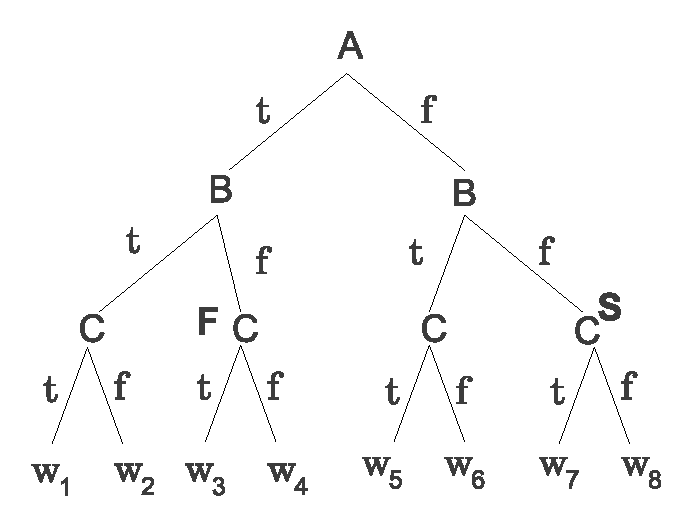
\includegraphics[width=0.5\textwidth]{searchtree}
	\caption{A search tree for the CNF $\Delta =\{\{\neg A,B\},\{\neg B,C\}\}$.}
	\label{fig:searchtree}
\end{figure}

\subsubsection{Depth-search-first algorithm}

\begin{algorithm}
\textsc{Depth-first-search}(CNF $\Delta$,depth $d$):\\
\uIf{$\Delta=\{\}$}{
	\bf{return \{\}}.
}
\uElseIf{$\{\}\in \Delta$}{
	\textbf{return} \textsc{unsatisfiable}
}
\uElseIf{\textsc{\textbf{L}}$=$\textsc{Depth-first-search}$(\Delta |P_{d+1},d+1)\neq$\textsc{unsatisfiable}}{
	\textbf{return} \textbf{L} $\cup$ $\{P_{d+1}\}$
}
\uElseIf{\textsc{\textbf{L}}$=$\textsc{Depth-first-search}$(\neg \Delta |P_{d+1},d+1)\neq$\textsc{unsatisfiable}}{
	\textbf{return} \textbf{L} $\cup$ $\{\neg P_{d+1}\}$
}
\Else{\textbf{return} \textsc{unsatisfiable}}
\caption{Depth-first-search algorithm\label{dpll}}
\end{algorithm}    

The Davis-Putnam-Logemann-Loveland (DPLL) \cite{dpll} algorithm is the base of all modern SAT solvers. Many refinements have been made to this algorithm over the last decade, which have been significant enough to change the behaviour of the algorithm, but it is still important to know it for understanding modern solvers. Figure ~\ref{fig:searchtree} shows a search tree with three variables. We can observe that the leaves of this tree and in one-to-one correspondence with all the possible true assignments of variables involved, so testing satisfiability can be viewed as searching for a leaf node that satisfies the CNF. Another important observation is that the depth of the tree is $n$, where $n$ is the number of boolean variables, so performing a depth-first-search would be best to explore the tree. Algorithm ~\ref{dpll} performs a depth-first-search, which is the base of the DPLL algorithm, using the conditioning operator on CNFs to remove clauses or reduce their size.

Consider the CNF:
\[\Delta=\{\{\neg A,B\},\{\neg B,C\}\},\]
and the search node labelled with \textbf{F} in Figure ~\ref{fig:searchtree}. At this node, Algorithm ~\ref{dpll} will condition $\Delta$ on literals $A,\neg B$, leading to:
\[\Delta |A,\neg B=\{ \{\textbf{false},\textbf{false}\},\{\textbf{true},C\}\}=\{\{\}\}.\]
The algorithm will detect that at this internal node that there is a contradiction, hence concluding that neither $w3$ or $w4$ are models of $\Delta$, without having to visit them explicitly. The algorithm can also detect success at internal nodes, implying that all assignments from that particular node are models of the CNF.

\subsubsection{Unit Resolution}

\begin{figure}[h!]
	\centering
		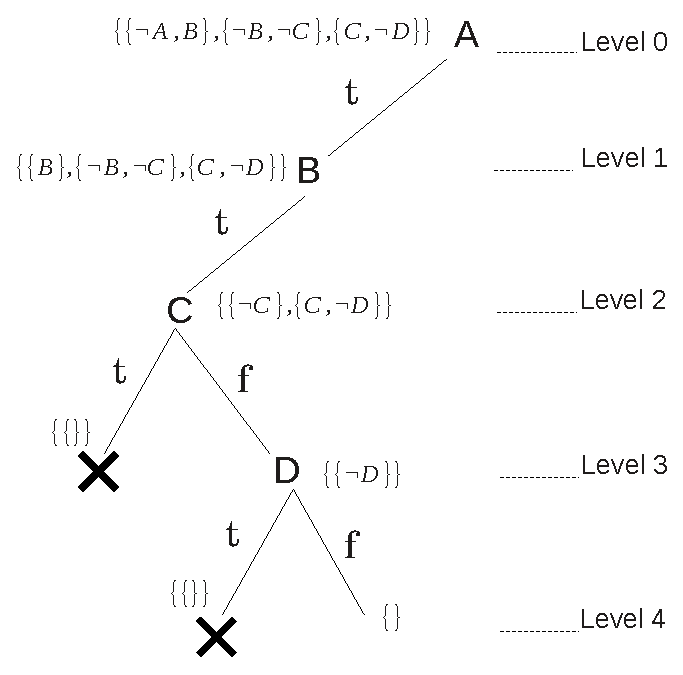
\includegraphics[width=0.5\textwidth]{termination_tree}
	\caption{A termination tree, where each node is labelled by the corresponding CNF. The last node visited during the search is labelled with \{\}. The label X indicates the detection of a contradiction at that node.}
	\label{fig:searchtree}
\end{figure}

Consider the tree of Figure ~\ref{fig:searchtree} and the CNF:
\[\Delta=\{\{\neg A,B\},\{\neg B,\neg C\},\{C,\neg D\}\}.\]
Consider also the node at Level 1, which results from setting variable A to \textbf{true}, and its corresponding CNF:
\[\Delta |A=\{\{B\},\{\neg B,\neg C\},\{C,\neg D\}\}.\]
Algorithm ~\ref{dpll} cannot declare early success or early failure, because the CNF is neither empty, nor contains the empty clause, reason why it keeps searching below Level 1 as shown in Figure \ref{fig:searchtree}. However, we will now show that by using unit resolution, we can declare success success and end the search at Level 1.

The \textit{unit resolution technique} (also called \textit{unit propagation}) is very simple: Before we check tests for success or contradictions, we first collect all unit clauses. Then we assume that the variables which make these clauses unit are set to satisfy the unit clauses. Finally we simplify the CNF and check for success or failure.

To incorporate unit resolution into Algorithm \ref{dpll}, we will introduce a function \textsc{unit-resolution}, which applies to a CNF $\Delta$ and returns two results:
\begin{itemize}
	\item \textbf{I}: a set of literals that are either present as unit clauses in $\Delta$, or were derived from $\Delta$ by unit resolution.
	\item $\Gamma$: a new CNF which results from conditioning $\Delta$ on literals \textbf{I}.
\end{itemize}
For example, if the CNF
\[\Delta=\{\{\neg A,\neg B\},\{B,C\},\{\neg C,D\},\{A\}\},\]
then $\textbf{I}=\{A,\neg B,C,D\}$ and $\Gamma=\{\}$. Moreover, if
\[\Delta=\{\{\neg A,\neg B\},\{B,C\},\{\neg C,D\},\{C\}\},\]
then $\textbf{I}=\{C,D\}$ and $\Gamma=\{\{\neg A,\neg B\}\}$.

\subsubsection{DPLL algorithm}

\begin{algorithm}
$(\textbf{I},\Gamma)=\textsc{unit-resolution}(\Delta)$\\
\uIf{$\Gamma=\{\}$}{
	\bf{return \textbf{I}}.
}
\uElseIf{$\{\}\in \Gamma$}{
	\textbf{return} \textsc{unsatisfiable}
}
\Else{
	choose a literal $L$ in $\Gamma$\\
	\uIf{$\textbf{\textsc{L}}=\textsc{dpll}(\Gamma |L) \neq \textsc{unsatisfiable}$}{
		\textbf{return} \textbf{L} $\cup$ \textbf{I} $\cup$ $\{L\}$	
	}
	\uElseIf{$\textbf{\textsc{L}}=\textsc{dpll}(\Gamma |\neg L) \neq \textsc{unsatisfiable}$}{
		\textbf{return} \textbf{L} $\cup$ \textbf{I} $\cup$ $\{\neg L\}$	
	}
	\Else{
		\textbf{return} \textsc{unsatisfiable}
	}
}
\caption{DPLL(CNF $\Delta$): returns a set of literals or \textsc{unsatisfiable}\label{dpllplus}}
\end{algorithm}    

The DPLL algorithm (Algorithm \ref{dpllplus}) is a refinement of the depth-first-search algorithm. The first change made is that it adds unit resolution in line 1. Also, we no longer assume that variables are examined in the same order as we go down the search tree and we no longer assume that a variable is set to \textbf{true} and then to \textbf{false}. The choice of a literal $L$ on line 7 can have a dramatic impact on the running time of DPLL. This is where inference comes into play when solving a SAT instance with a DPLL based algorithm, heuristics and random factors are commonly used at this point. 

\subsubsection{Chronological backtracking}

When we detect a conflict at level $l$ of the search tree, we have to rewind back to level $l-1$, undoing all assignments done in the process. Then we try another value at level $l-1$, if none remains  to be tried, we then go back further to level $l-3$, and so on. If we ever reach level $0$ and each value there leads to a contradiction, we will know that the CNF is inconsistent. This type of backtracking is called \textit{chronological backtracking}, because the we move back in the same order we got there; one level at a time. 

\subsubsection{Non-Chronological backtracking}

The problem with this type of backtracking, which is the one used in the DPLL algorithm, is that contradictions (when an assignment we have done does not satisfy the CNF) that trigger the backtrack often have valuable information. Such information could lead us to learn new clauses and backtrack more levels than just one, thus saving time in the search. For example, let's say that we have a CNF $\Delta$ with variables $A,B,C,D$. Let's us also say that, because of the clauses in $\Delta$, the CNF will always be inconsistent when $A$ is set to \textbf{true}. Unfortunately, the DPLL algorithm might not realise this beforehand, because it uses unit resolution which is not refutation complete. So the algorithm might only conclude that $A$ set to \textbf{true} will not satisfy $\Delta$ after assigning all possible values to $B,C,D$. If we could detect that $A$ is not part of any solution, we could avoid going any further in that branch of the search tree and learn that information as a clause. This is the reason why conflict driven clauses \cite{cdcl} were introduced to SAT solving algorithms.


\subsection{PaMiraXT}

PaMiraXT \cite{SLB09} is one of the first attempts to use a shared clause database in a parallel SAT solver.

\subsection{Plingeling}

\subsection{


%%%%%%%%%%%%%%%%%%%%%%%%%%%%%%%%%%%%%%%%%%%%%%%%%%%%%%%%%%%%%%%%%%%%%%%%%%%%%%%%
% Step 12: Here's the main part of your research project. We can't tell
% you what to write here... that's your job.
% 
%%%%%%%%%%%%%%%%%%%%%%%%%%%%%%%%%%%%%%%%%%%%%%%%%%%%%%%%%%%%%%%%%%%%%%%%%%%%%%%%
\chapter{Important stuff...}\label{chap:contributions}

\section{Cache performance in simple parallel-shared-memory programs}
The main motivation behind this work is our experimental evidence that when threads in different cores share memory, the cache performance improves compared to having threads with its own memory. Our first experiment will be a program that performs simple arithmetic operations on a big matrix. We will have two instances for this experiment. The first will be different threads performing the same arithmetic operations over the same matrix (hence yielding the same result), but every thread will hold its own copy of the big matrix. The second instance will be the same experiment, but this time the different threads will perform the arithmetic operations over the same matrix (regarding physical memory location). For this experience, we will only use read-only operations over the matrix, to keep concurrency problems out of the equation.

To measure cache performance we will use the linux tool \textit{perf}. Table \ref{matrix} shows...

\section{Cache performance of parallel SAT solvers}

\subsection{Barcelogic}

\subsection{Plingeling}

\section{A parallel portfolio approach SAT solver with physicaly shared clause database: AzuDICI}

\subsection{General outline}

\subsection{Data structures involved}

\subsection{Propagation}

\subsection{Experimental results} 

%%%%%%%%%%%%%%%%%%%%%%%%%%%%%%%%%%%%%%%%%%%%%%%%%%%%%%%%%%%%%%%%%%%%%%%%%%%%%%%%
% Step 13: Add a conclusions chapter
%
% 
%%%%%%%%%%%%%%%%%%%%%%%%%%%%%%%%%%%%%%%%%%%%%%%%%%%%%%%%%%%%%%%%%%%%%%%%%%%%%%%%
\chapter{Conclusions}\label{chap:conclusion}

%%%%%%%%%%%%%%%%%%%%%%%%%%%%%%%%%%%%%%%%%%%%%%%%%%%%%%%%%%%%%%%%%%%%%%%%%%%%%%%%
% Step 14: Work out the bibliography
%
% 
%%%%%%%%%%%%%%%%%%%%%%%%%%%%%%%%%%%%%%%%%%%%%%%%%%%%%%%%%%%%%%%%%%%%%%%%%%%%%%%%
% Tips: 
%
% For named.bst, if I add a~\cite*{} it will add all the references I
% have in the bibliography file (whether they are referenced in the
% document or not)
%%%%%%%%%%%%%%%%%%%%%%%%%%%%%%%%%%%%%%%%%%%%%%%%%%%%%%%%%%%%%%%%%%%%%%%%%%%%%%%%
\bibliographystyle{plain}
\bibliography{biblio}

\end{document}
